\documentclass[11pt, oneside]{article}  
\usepackage[margin=0.5in]{geometry} % Margins
\usepackage[ampersand]{easylist} % Bullets for lists
\usepackage[bottom]{footmisc}  % Glue footnotes to bottom
\usepackage{listings}
\usepackage{amsmath}
\usepackage{float}
\usepackage{array,mathtools}

\newcommand*{\carry}[1][1]{\overset{#1}}
\newcolumntype{B}[1]{r*{#1}{@{\,}r}}

\title{Homework 4\\UCLA-CS180-S18}
\author{Quentin Truong}


\begin{document}
\maketitle
\pagenumbering{arabic}


%========================================================
\section{Question 1}
a) 19 \newline
b) 2 \newline
c) see picture \newline
\begin{figure}[ht]
\begin{center}
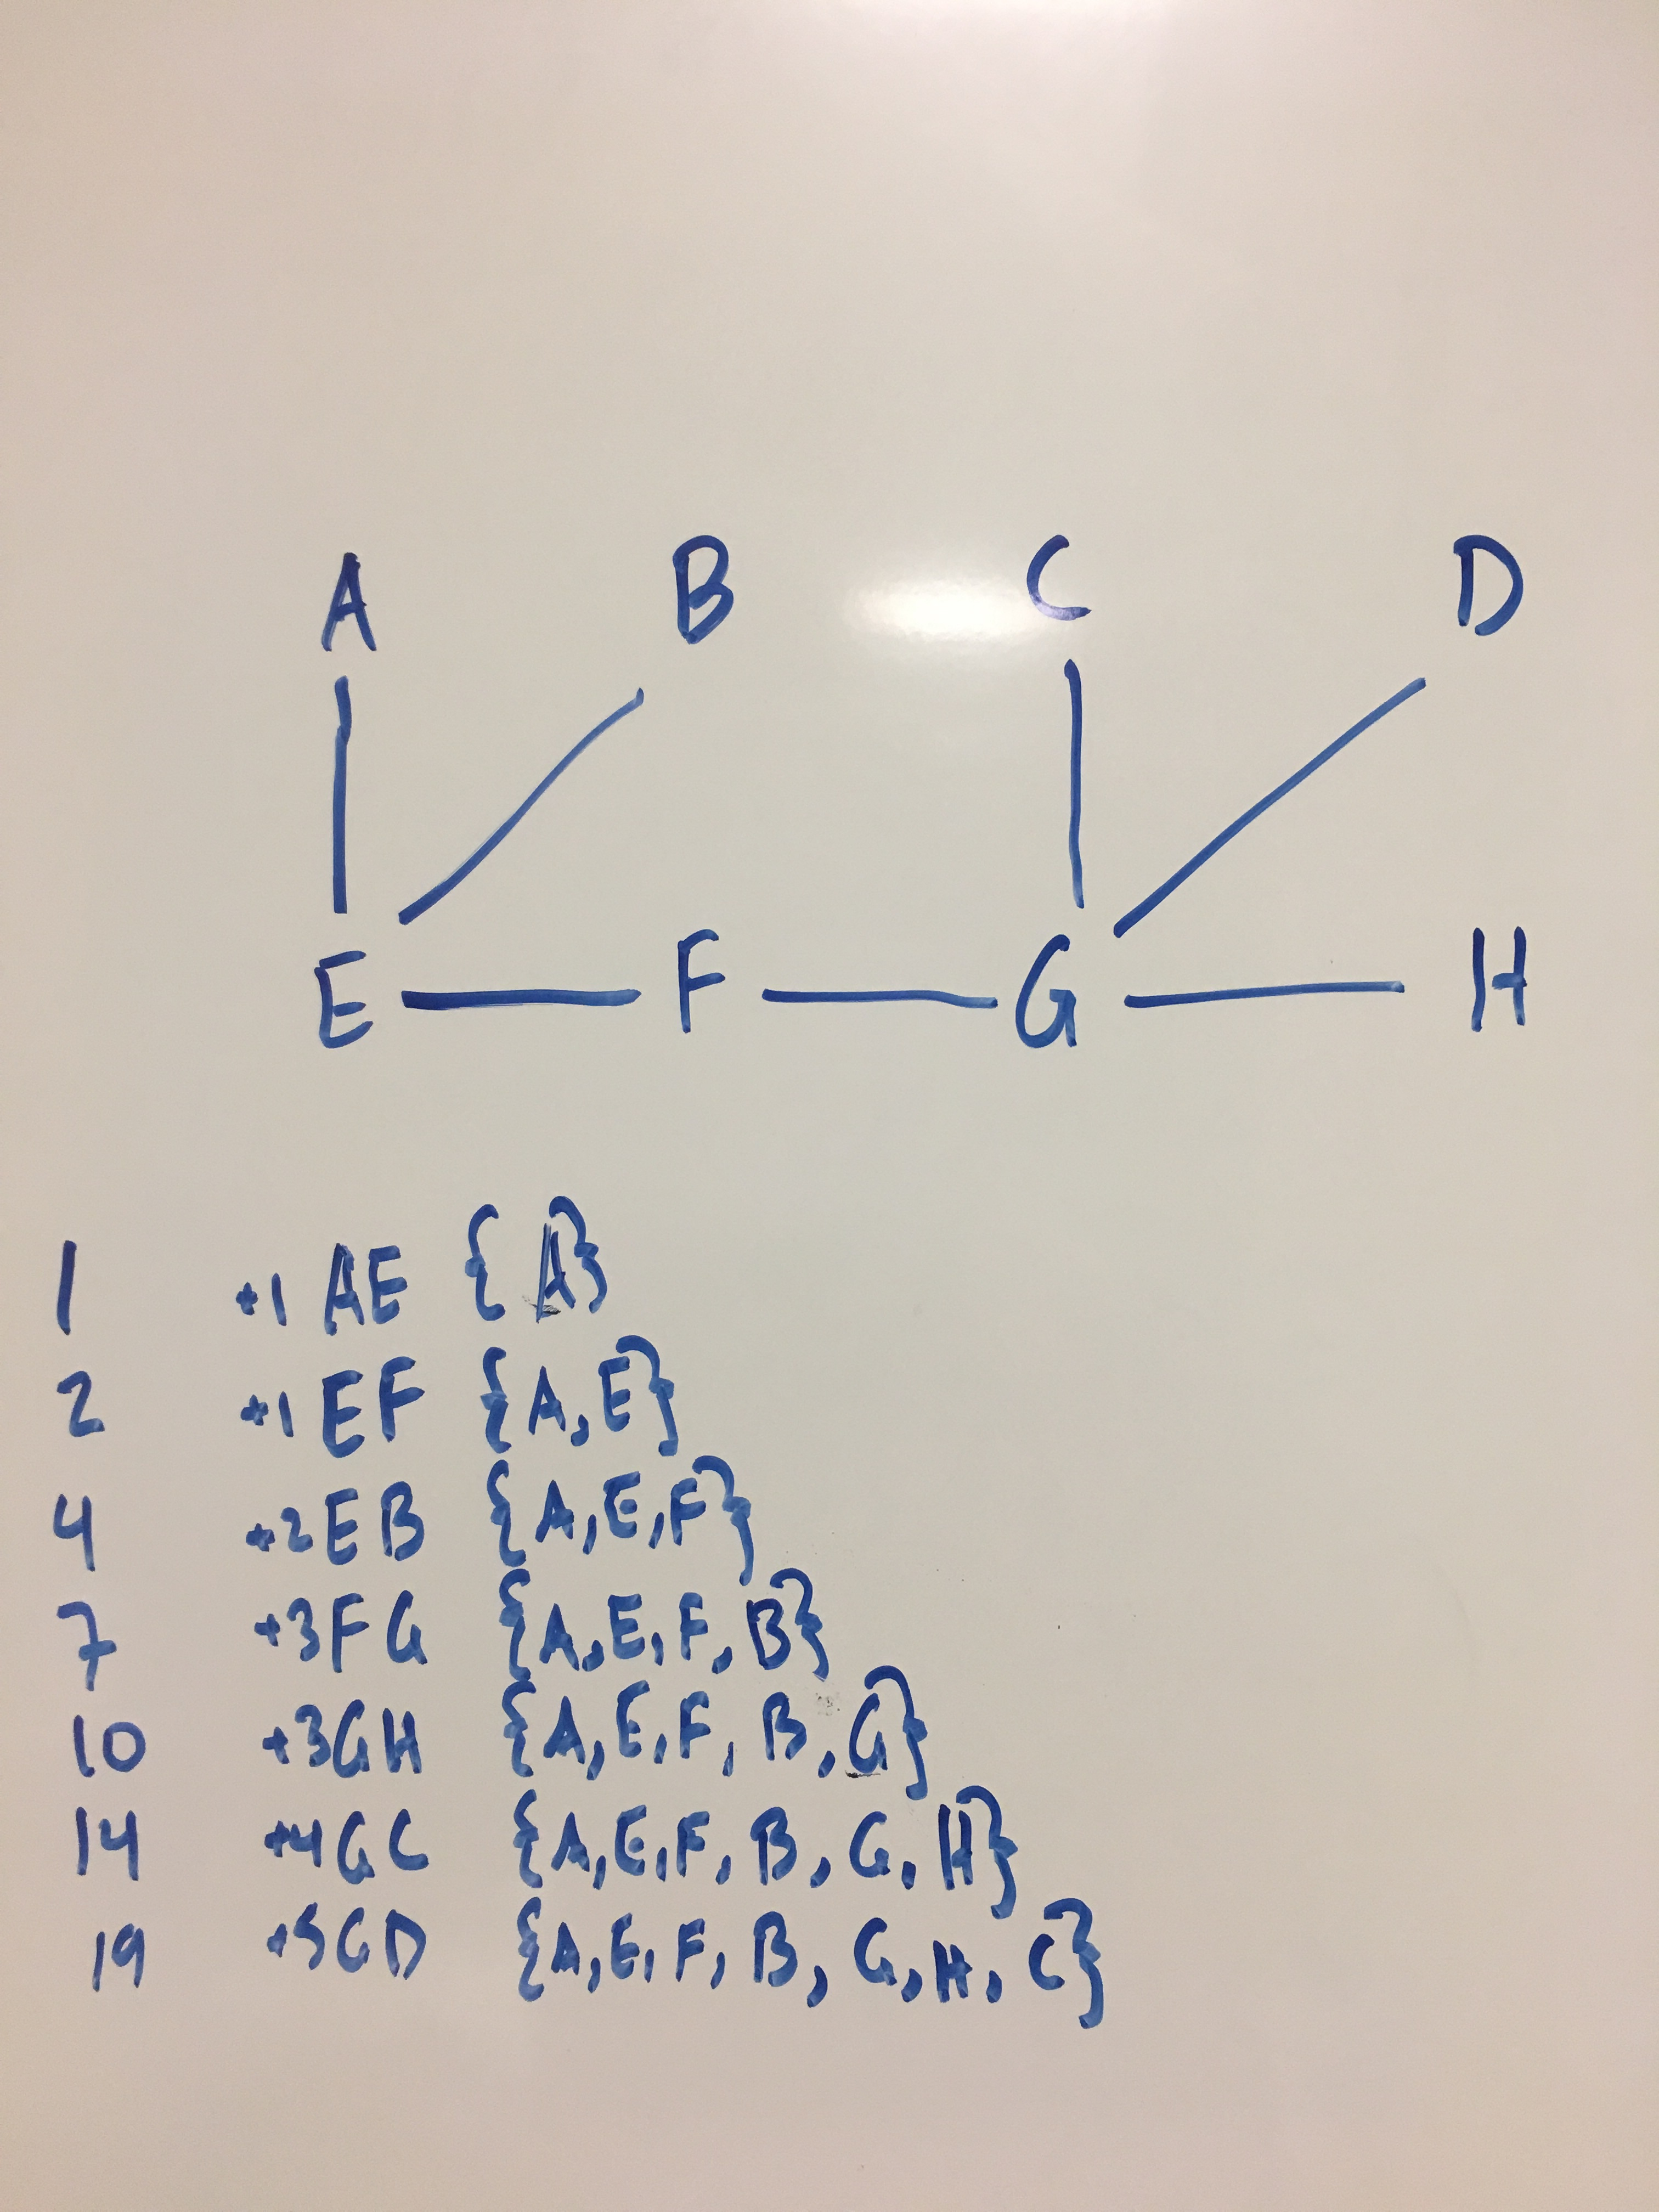
\includegraphics[scale=0.1]{unnamed.jpg}
\end{center}
\end{figure}

\clearpage
%========================================================

%========================================================
\section{Question 2}

This is proven by the cut property. We arbitrarily choose either of the two connected components created from removing edge e from graph T to be the cut. We check every edge in G leaving the cut. If e is not a minimum weight crossing the cut, then T is no longer an MST. This is because a minimum edge must be used to cross any cut according to the cut property. The algorithm checks precisely this - the algorithm finds the cut and compares the cost of every edge leaving the cut against the updated edge. \newline

\begin{lstlisting}
function check_if_still_mst(G, T, e)
    remove(T, e)
    // O(E) to remove edge from graph

    cut = BFS(T, e[0])
    // returns set of vertices in connected component in O(V+E) -> O(E) bc MST

    for src in cut
        for dest in G[src]
            // reaches this point a maximum of E times bc only that many edges
            if dest not in cut AND cost(src, dest) < cost(e) 
                // O(1) check if in set
                // O(1) to check cost
                return false

    return true

function remove(graph, edge)
    graph[edge[0]].remove(edge[1])
    graph[edge[1]].remove(edge[0])
    // O(n) to remove element from list
\end{lstlisting}


\clearpage
%========================================================

%========================================================
\section{Question 3}

items is a list of projects, each with goodwill (v), student-athlete requirement (a), and buses (b) \newline
limit\_A is the number of student-athletes who want to volunteer \newline
limit\_B is the number of buses available \newline

\begin{lstlisting}
function knapsack_two_constraints(items, limit_A, limit_B)
    value = 3D array with each value initialized to 0
    sol = 3D array with each value initialized to empty set

    for i in [1, ..., len(items)]
        for a in [1, ..., limit_A]
            for b in [1, ..., limit_B]
                if i.a <= a AND i.b <= b 
                AND i.v + value[i - 1, a - i.a, b - i.b] > value[i - 1, a, b]
                    value[i, a, b] = i.v + value[i - 1, a - i.a, b - i.b]
                    sol[i, a, b] = {i} union sol[i - 1, a - i.a, b - i.b]
                else
                    value[i, a, b] = value[i - 1, a, b]
                    sol[i, a, b] = sol[i - 1, a, b]
                    
    return value[len(items), limit_A, limit_B], sol[len(items), limit_A, limit_B]
\end{lstlisting}

\clearpage
%========================================================

%========================================================
\section{Question 4}

Basically, we are just saying that the number of subsets is the number of subsets you can create using this item at this weight + number of subsets you can create without this item at this weight

\begin{lstlisting}
function count_subsets(items, W)
    count = 2D array with each value initialized to 0

    for i in [1, ..., len(items)]
        for w in [1, ..., W]
            if w - i.w >= 0
                count[i, w] = 1 + count[i - 1, w - i.w] + count[i - 1, w]
            else
                count[i, w] = count[i - 1, w]

    return count[len(items), W]
\end{lstlisting}

\clearpage
%========================================================

\end{document}